
%sudo apt-get install texlive-bibtex-extra
%Word counts: pdftotext WBVFM_IntroPar.pdf - | wc -w
\documentclass{article}\usepackage[]{graphicx}\usepackage[]{color}
%% maxwidth is the original width if it is less than linewidth
%% otherwise use linewidth (to make sure the graphics do not exceed the margin)
\makeatletter
\def\maxwidth{ %
  \ifdim\Gin@nat@width>\linewidth
    \linewidth
  \else
    \Gin@nat@width
  \fi
}
\makeatother

\usepackage{Sweave}


\usepackage{float}
\usepackage{wrapfig}
\usepackage{hyperref}
\usepackage{authblk}
\usepackage[backend=bibtex, style=nature, citestyle=authoryear]{biblatex}
\bibliography{WBVFM_IntroPar}
\newenvironment{knitrout}{}{}  %just a dummy environment
\makeatletter
\newcommand\gobblepars{%
    \@ifnextchar\par%
        {\expandafter\gobblepars\@gobble}%
        {}}
\makeatother



\author[1]{Daniel Runfola\thanks{dsmillerrunfol@wm.edu}}
\author[1]{Ariel BenYishay\thanks{abenyishay@wm.edu}}
\author[2]{Jeff Tanner\thanks{jtanner@worldbank.org}}
\author[3]{Graeme Buchanan\thanks{graeme.buchanan@rspb.org.uk}}
\author[4]{Jyothy Nagol\thanks{jnagol@umd.edu}}
\author[5]{Matthias Leu\thanks{mleu@wm.edu}}
\author[1]{Seth Goodman \thanks{smgoodman@wm.edu}}
\author[1]{Rachel Trichler\thanks{rbtrichler@wm.edu}}
\author[1]{Rob Marty\thanks{ramarty@email.wm.edu}}

\affil[1]{Institute for the Theory and Practice of International Relations, The College of William and Mary}
\affil[2]{Independent Evaluation Group, World Bank}
\affil[3]{Center for Conservation Science, Royal Society of Birds}
\affil[4]{Global Land Cover Facility, University of Maryland}
\affil[5]{Department of Biology, The College of William and Mary}

\renewcommand\Authands{ and }

\title{A top-down approach to estimating spatially hetereogeneous impacts of development aid on vegetative carbon sequestration}
\date{\vspace{-5ex}}
\IfFileExists{upquote.sty}{\usepackage{upquote}}{}
\begin{document}
\begin{knitrout}


\maketitle 
\begin{flushleft}
\textbf{Short Title}: Estimating impacts of aid on carbon sequestration\\
\textbf{Keywords}: International Aid, Carbon Sequestration, Causal Identification, Heterogeneous Effects\\
\textbf{Words in Abstract:} 150\\
\textbf{Words in Manuscript:} 3000\\
\textbf{Number of References:} 30\\
\textbf{Number of Figures and Tables:} 10\\
\textbf{Corresponding Author}:\\
Dr. Daniel Runfola\\
Institute for the Theory and Practice of International Relations, \emph{AidData}
Email: dsmillerrunfol@wm.edu
Telephone: 508.316.9109
Fax: 757.221.4650
\end{flushleft}

\newpage
\section{Abstract}
  Since 1945, over \$4.9 trillion dollars of international aid has been allocated (\cite{tierney_more_2011}).
 To date there have been no estimates of the regional impact of this aid on the carbon cycle.  
 We apply a geographically explicit matching method (\cite{andam_measuring_2008}) to estimate the impact of World Bank projects implemented between 2000 and 2010 on sequestered carbon, using a novel and publically available dataset of 47,084 World Bank project locations \footnote{http://aiddata.org/level1/geocoded/worldbank}. 
 Considering only carbon sequestered due to fluctuations in vegetative biomass caused by World Bank projects, we estimate a global net positive increase in sequestration totaling 1,398,229 tonnes. 
However, we illustrate the apparent effectiveness of environmental safeguards (\cite{laurance_reducing_2015}) implemented by the World Bank are variable across different geographic contexts.  
We argue that subnational data can be helpful in the identification of these heterogeneous impact effects, and highlight the considerable methodologic barriers which still exist.

\newpage
\section{Introduction}



The Introduction should summarize briefly the background and aims, and end with a brief statement of what has been achieved by the work.

\section{Methods}
This section should contain sufficient detail so that all procedures can be repeated (in conjunction with cited references). Where specific equipment and materials are named, the manufacturer’s name, city and country should be given (generally in parentheses after first mention).

\section{Results}
The Results section should present the experiments that support the conclusions to be drawn later in the Discussion. The Results section should conform to a high standard of rigour. Extended lines of inference, arguments or speculations should not be placed in the Results.

\begin{wrapfigure}[20]{r}{0.65\textwidth}\centering
%\begin{minipage}{.75\textwidth}
\begin{Schunk}

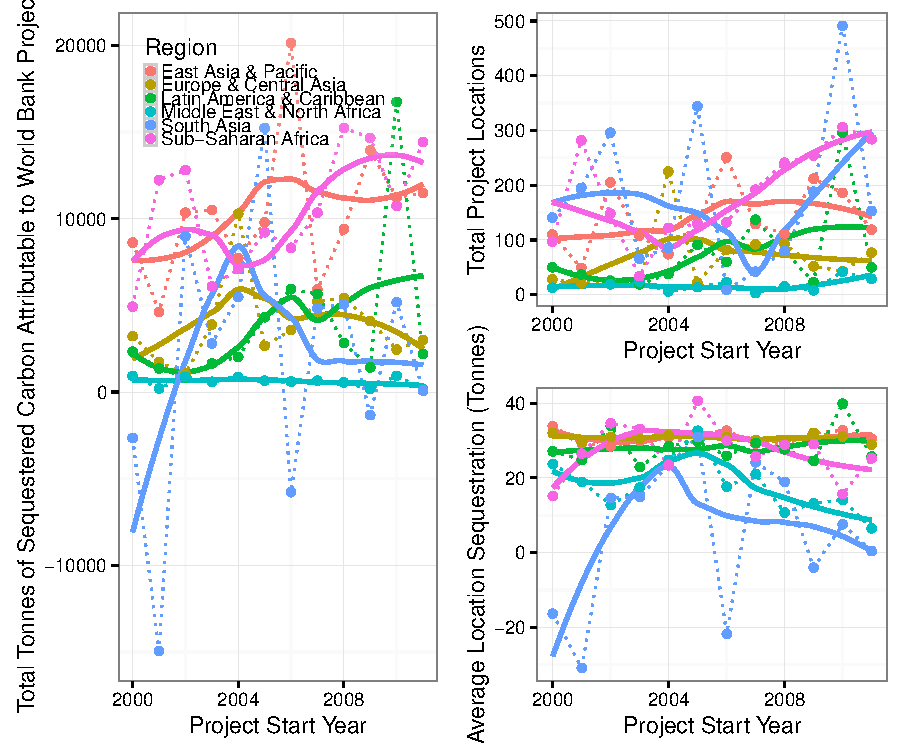
\includegraphics[width=\maxwidth]{figure/Fig1-1} \end{Schunk}
%\end{minipage}
\end{wrapfigure}  

\section{Discussion}
The Discussion section should be separate from the Results section. It allows authors to propose their interpretation of the results, and to suggest what they mean in a wider context. It should end with a clear statement of the main conclusions of the research, and a clear explanation of their importance and relevance to applied conservation and/or policy.

\section{Acknowledgements}
The authors would like to acknowledge the government of Sweden and the World Bank Independent Evaluation Group for partially funding this research.  This work was performed in part using computational facilities at the College of William and Mary which were provided with the assistance of the National Science Foundation, Virginia Port Authority, Virginia's Commonwealth Technology Research Fund, and the Office of Naval Research.  The authors would also like to thank Scott Stewart, Alex Kappel, Miranda Lv, Doug Nicholson, and Vinay Vijayan for their valuable contributions and insights.


\newpage
\section{References}
%Need to ensure formatting is correct -
%http://endnote.com/downloads/style/conservation-letters
%Limited to 40 references
\printbibliography



\end{knitrout}
\end{document}
